\section{LC-Modulator als DOE}
\subsection{Berechnung der Pixelgröße}
\subsubsection{Theorie}
Zur Bestimmung der Breite eines Pixels innerhalb des LC-Modulators wird mit der Formel eines Gitters gerechnet, da ein LC-Modulator dasselbe Beugungsbild aufweißt.
\begin{align}
	g\sin{\alpha} = m\lambda
	\label{gbestimm}
\end{align}
Dabei stellt g die Gitterkonstante, $\alpha$ den Winkel zwischen der nullten und m.ten Beugungsordnungen, m die entsprechende Beugungsordnung und $\lambda$ die Wellenlänge des Lasers ($\lambda = 650nm$) dar.
Die Bestimmung von $\alpha$ kann aus der Optik durch
\begin{align}
	\alpha \approx \frac{d}{2f}
	\label{abestimm}
\end{align}
berechnet werden. Dabei ist d der Abstand zweier gleicher höherer Ordnungen. 
\subsubsection{Aufbau}
Der Aufbau zur Berechnung der Pixelgröße ist in \cref{421} dargestellt.
Zuerst wird der Laser auf einen LC-Modulator gerichtet, welcher in dem Abstand der Brennweite der Linse ($f = 16cm$) von der Linse entfernt steht. Zwischen der Linse und dem LC-Modulator ist ein Analysator. Hinter der Linse ist im Abstand ihrer Brennweite ein Schirm aufgestellt, um die Beugungsordnungen messen zu können. 
\begin{figure}[h!]
	\centering
	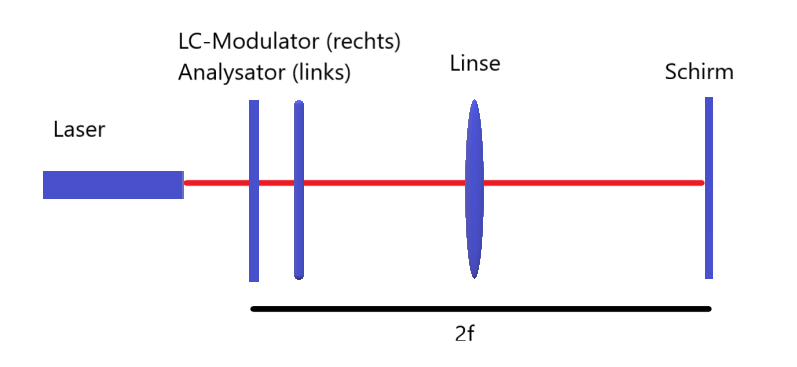
\includegraphics[scale = 1]{4.2.1-Aufbau.png}
	\caption{Aufbau zur Bestimmung der Pixelgröße}
	\label{421}
\end{figure}
\subsubsection{Auswertung}
Um \cref{gbestimm} möglichst genau zu berechnen wurde bei der Berechnung von \cref{abestimm} der Abstand der siebten Ordnungen benutzt, um d zu messen. Dieser Abstand wurde mittels eines Lineals gemessen. Aus diesen Berechnungen kann die Gitterkonstante bestimmt werden $g = 0,0029cm$.
\subsubsection{Unsicherheiten}
Die Unsicherheiten für g müssen noch geschrieben werden.
\subsubsection{Diskussion}
Die Diskussion mit dem Aufgabenteil 1 muss auch noch geschrieben werden.

\subsection{Intensitätsverteilung in den Beugungsordnungen des unadressierten Displays}
\subsubsection{Theorie}
Eine LCD-Zelle besitzt eine Untermodulation. Dies ist deshalb der Fall, da in einem einfachen Pixel es einen transparenten Anteil gibt, sowie einen Lichtundurchlässigen Anteil. Die Modulation wird durch das Gitter beschrieben, welches im vorherigen Aufgabenteil behandelt wurde. Die Untermodulation wird durch die Substruktur im Pixel erzeugt. An dieser Stelle wird der duty cycle definiert. Dieser beschreibt das Verhältnis zwischen transparentem und lichtundurchlässigem Teil. Danach kann auf einen Füllfaktor geschlossen werden für den transparenten Teil des Pixels.
\subsubsection{Aufbau}
Der Aufbau zur Berechnung des Füllfaktors der LCD-Zelle ist in \cref{422} dargestellt. Zuerst wird der Laser, welcher eine zusätzlich integrierte Aufweitungsoptik besitzt auf das LCD-Display gerichtet. Danach wird ein Analysator in den Strahlengang geführt. Statt einem Schirm wird die Auswertung mit einem Intensitätsmessgerät durchgeführt.
\begin{figure}[h!]
	\centering
	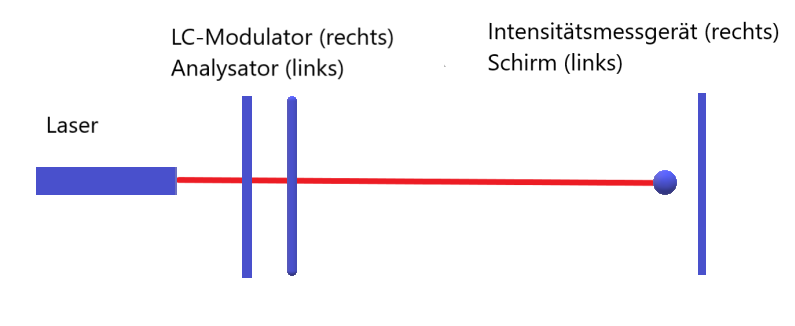
\includegraphics[scale = 1]{4.2.2-Aufbau.png}
	\caption{Aufbau zur Bestimmung des Füllfaktors der LCD-Zellen}
	\label{422}
\end{figure}
\subsubsection{Auswertung}
Im weiteren wurden die ersten zehn Beugungsordnungen in horizontaler und vertikaler Ebene gemessen. Die Messwerte sind in \cref{horiz} zu sehen.
\begin{figure}[h!]
	\centering
	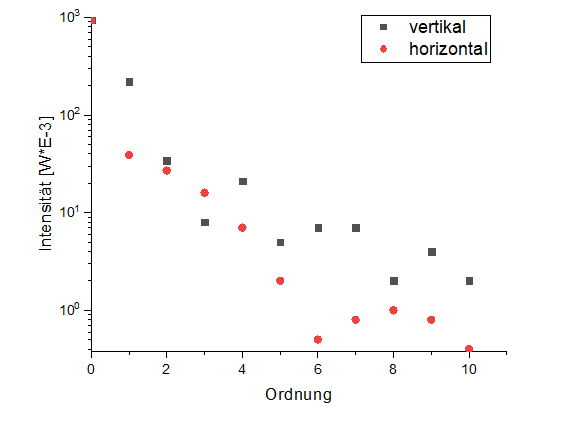
\includegraphics[scale = 1]{horizundvertik.png}
	\caption{Intensitätsverteilung der horizonatlen und vertikalen Beugungsordnungen}
	\label{horiz}
\end{figure}
Aus den Messwerten kann auf den duty cycle geschlossen werden, sowie auf den Füllfaktor des transparaneten Teils der LCD-Zelle

\subsection{Aufnahme von verschiedenen Beugungsbildern mittels der Kamera}
\subsubsection{Theorie}
\subsubsection{Aufbau}
Der Aufbau in \cref{423} ist identisch mit dem Aufbau in \cref{421} mit dem Unterschied, dass statt des Schirms eine Kamera integriert wurde.
\begin{figure}[h!]
	\centering
	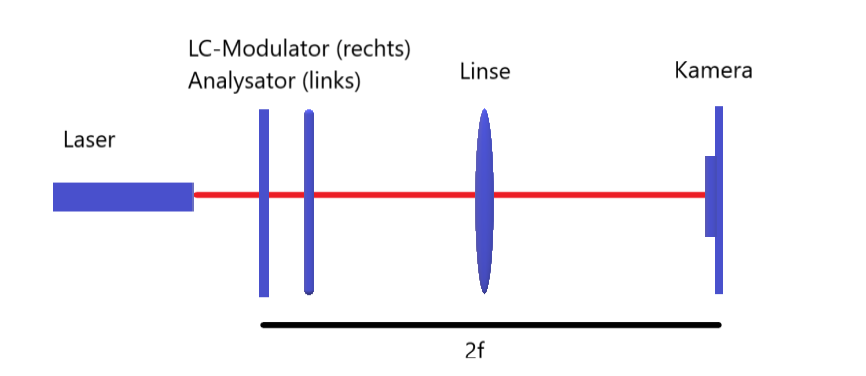
\includegraphics[scale = 1]{Kamera111.png}
	\caption{Aufbau zur Aufnahme von Beugungsbildern, die von dem LC-Modulator erzeugt werden mit Hilfe einer Kamera.}
	\label{423}
\end{figure}
\subsubsection{Auswertung}
In diesem Teil werden Beugungsbilder verschiedener DOE's aufgenommen. Darunter befinden sich der Einzelspalt, der Doppelspalt und das Gitter. Bei dem Einzelspalt weren zwei verschiedene Strukturgrößen benutzt.

\subsubsection{Unsicherheiten}
\subsubsection{Diskussion}




